Wie bereits im Kapitel 3.1.2 beschrieben, muss durch die Verwendung von OSS der konkrete Prozess innerhalb des Beispielprojektes angepasst werden. Die erste notwendige Anpassung erfolgt mittels einer Überprüfung der verwendeten Lizenzmodelle basierend auf einer manuellen Checkliste durch die entsprechenden Entwickler. Durch das strukturierte und mehrmalige Arbeiten mit einer manuellen Checkliste entsteht eine Routine für das Entwicklerteam innerhalb des gesamten Softwareentwicklungsprozesses.\\\\ Softwarekomponenten sind oftmals stark miteinander verschachtelt und enthalten zudem viele transitive Abhängigkeiten, wodurch das Ziel verfolgt wird, mit der manuellen Checkliste eine gemeinsame Basis, Effizenz und eine Zeitersparnis zu schaffen, da nur das Lizenzmodell betrachetet wird, was in diesem Moment verwendet werden soll. Dieser Schritt entspricht zwar nicht der gängigen DevOps-Kultur einen möglichst hohen Grad an Automatisierung zu erlangen, jedoch kann bereits durch einen kurzen manuellen Check 'gefährliche' und 'ungefährliche' Lizenzmodelle voneinander unterschieden werden bevor eine langwierige Entwicklung stattfindet. Ferner ist an diesem anfänglichen Entwicklungszeitpunkt die Überprüfung mittels einer automatisierten Checkliste bedenklich, da mit der Software zunächst vorrangig expermentiert wird und eine vollständige Integration in die bestehende Anwendung somit nicht feststeht. Andernfalls müsste jede heruntergeladene OSS direkt in das Softwareentwicklungsprozess integriert werden, um diese anschließend automatisiert überprüfen zu lassen. Die Folgen wären ein Verlust von wichtigen Ressourcen, Effizenz und Zeit.\\\\ Ziel des Einsatzes der manuellen Checkliste ist es, sowohl die technische als auch juristische Faktoren bei der Verwendung von OSS zu berücksichtigen und ein gemeinsames Verständnis zu erreichen. Innerhalb der kommerziellen Softwareentwicklung stellt dies eine große Herausforderung dar. Softwarearchitekten haben oftmals eine starke funktionale und strukurelle Sichtweise und wenig Affinität zu Lizenztexten und benötigen daher Hilfe bei der Auswahl von OSS-Komponenten. Menschen mit juristischen Hintergrund,  hingegen haben ein Verständnis für Lizenzen und Recht, allerdings können sie, die tatsächliche technische Ausprägung einer Softwarekomponente rechtlich nicht intepretieren. Benötigt wird eine aussagekräftige Entscheidungsgrundlage, die aufzeigt, ob der Einsatz einer bestimmten Komponente rechtlich zulässig ist. Darüber hinaus sollte bei der Bewertung der Lizenzmodelle auch die jewelige Nutzung der Komponenten berücksichtigt werden, die einen erheblichen Einfluss auf die zu erfüllenden Lizenzbedingungen haben kann. So ist beispielsweise die interne Nutzung oft unbedenklich und bedarf keiner Bedingungen, während eine Weitergabe viele Einschränkungen mit sich bringt. Die unten stehende manuelle Checkliste und die zugrunde liegenden Elemente wurden bereits innerhalb der msg systems ag als OSS-Guide erstellt worden und im Rahmen dieser Arbeit auf das Problemfeld erweitert und angepasst.
%Hier Fußzeile zu dem OSS-Guide von Ralf und Navina  
%Thesis von Navina nochmal lesen und paragraphen abändern

\subsubsection{Use Types}

Zunächst werden die 'Use Types' also die unterschiedlichen Nutzungarten erläutert. Diese geben Auskunft darüber, welche Bedinungen zu den jeweiligen Nutzungsarten erfüllt sein müssen. Die vorgestellten Szenarien dienen als jeweilige Ausgangssituation, während die Nutzungsarten die jeweilige Verwendung detailliert beschreiben. 

\paragraph{3.3.1.1. Auflistung der Nutzungsarten}

%Zweizeilig
% \newcommand\T{\rule{0pt}{4ex}}
% \newcommand\B{\rule[-3ex]{0pt}{0pt}}
%Vierzeilig
\newcommand\A{\rule{0pt}{7ex}}
\newcommand\C{\rule[-6ex]{0pt}{0pt}}
%Dreizeilig
\newcommand\D{\rule{0pt}{5ex}}
\newcommand\E{\rule[-4ex]{0pt}{0pt}}
%Sechszeilig
\newcommand\F{\rule{0pt}{9ex}}
\newcommand\G{\rule[-8ex]{0pt}{0pt}}

\begin{landscape}
\begin{longtable}[h]{|l|c|c||c|c|c|}
    \toprule
    \textbf{Use Types} & \textbf{Erklärung} & \textbf{Beispiel} & \textit{SZ 1} & \textit{SZ 2} & \textit{SZ 3} \\
    \midrule
    \hline
    \T format: source & \parbox{7cm}{Komponente wird im unverfälschten Quellformat geliefert} & WEB-INF/jquery.js & - & - & \checkmark \B \\
    \hline
    \T format: compiled & \parbox{7cm}{Komponente wird in kompiliertem Format bereitgestellt} & com/example/foo.class & - & \checkmark & \checkmark \B \\
    \hline
    \A dependency: optional  & \parbox{7cm}{Komponente wird bei Bedarf geladen, und das Produkt würde vernünftigerweise ohne sie funktionieren} & JDBC driver & \checkmark & - & - \C \\
    \hline
    \D dependency: mandatory & \parbox{7cm}{Komponente wird dynamisch/statisch geladen/verlinkt und das Produkt funktioniert nicht ohne sie} & Hibernate ORM & - & \checkmark & \checkmark \E \\
    \hline
    \A delivery: internal & \parbox{7cm}{Komponente wird intern verwendet, ohne dass sie an andere Rechtssubjekte weitergegeben wird (z. B. zeitlich begrenzte Komponenten)} & Gradle/Ant/Maven & \checkmark & - & - \C \\
    \hline
    \D delivery: distributed & \parbox{7cm}{Komponente wird an andere Rechtssubjekte verteilt (z.B. Laufzeitkomponenten)} & lib/example-1.2.3.jar & - & \checkmark & \checkmark \E \\
    \hline
    \T usage: local-call & \parbox{7cm}{Komponente (über Produkt) wird lokal zur Ausführung aufgerufen} & C:\textbackslash  Example\textbackslash example.jar & - & \checkmark & \checkmark \B \\
    \hline
    \A communication: process & \parbox{7cm}{Komponente wird aufgerufen von Produkt über direkten prozessinternen Mechanismus (Funktionsaufruf, Dispatch-Tabelle, usw.)} & component\_function() & \checkmark & \checkmark & \checkmark \C \\
    \hline
    \D bundling: standalone & \parbox{7cm}{Komponenten-Artefakte, die noch völlig eigenständig und als solche erkennbar sind} & example-1.2.3.jar & \checkmark & \checkmark & \checkmark \E \\
    \hline
    \A artifact: pristine & \parbox{7cm}{Alle Komponenten-Artefakte sind unverändert, d.h. genau so, wie sie ursprünglich vom vorgelagerten Hersteller erhalten wurden} & example-1.2.3.jar!com/example/foo.class & \checkmark & \checkmark & - \C \\
    \hline
    \T artifact: modified & \parbox{7cm}{Komponenten-Artefakte wurden hinzugefügt/ersetzt/entfernt} & example-1.2.3.jar!com
    /example/addon.class & - & - & \checkmark \B \\
    \hline
    \bottomrule
\caption{Auflistung der Nutzungsarten mit Beispielen und Szenarien}    
\end{longtable}
\end{landscape}

Insgesamt gibt es 14 zu beachtende Nutzungsarten, die in der Tabelle 2 dargestellt werden. Darüber hinaus wurde mittels der Tabelle 2, die dazugehörigen Erklärungen und ein Beispiel angegeben. Ob die jeweiligen  Nutzungstypen sich für das Beispielprojekt eignen, wurde anhand der beschriebenen Szenarien im Kapitel 3.2. unterschieden. Die Nutzungstypen wurden in sieben verschiedene Kategorien unterteilt: Format (format), Abhängigkeit (dependency), Auslieferung (delivery), Einsatz (usage), Kommunikation (communication), Bündelung (bundling) und Artifakte (artifact).

\subsubsection{Umfang und Ausprägung der Verpflichtungen}

Je nach Nutzungsart müssen verschiedene und festgelegte Verpflichtungen innerhalb eines vorgeschriebenen Rahmens erfüllt werden oder können unter bestimmten Bedingungen ausgeschlossen werden. \cite{tldr_legal_software_2012}Aufgrund dessen kann der Umfang der Verplichtung sich um eine Last, die der Nutzer erfüllen muss handeln oder um eine bestimmte Nutzungsart beziehen, indem einzelne Verpflichtungen erfüllt werden müssen oder die gesamte Nutzung ausgeschlossen wird. 

\paragraph{3.3.2.1. Umfang der Verpflichtungsarten} $~$
Der Umfang der Verpflichtungen und deren genaue Erklärung und Zweck wurde in der Tabelle 3 festgehalten. \\

\begin{table}
\begin{center}    
\begin{tabular}[h]{|r|c|l|}
    \hline\hline
    Verpflichtungsumfang & Zweck & Erklärung \\
    \hline\hline
    \A \parbox{4cm}{OBLIGATION (OBL)} & \parbox{5cm}{Eine Bedingung muss erfüllt werden, um die Lizenzbedingungen zu erfüllen} & \parbox{5cm}{Eine Lizenzvereinbarung enthält mehrere Bedingungen, die erfüllt werden müssen} \C \\
    \hline
    \F \parbox{4cm}{NOT OBLIGATION SINGLE (NOS)} & \parbox{5cm}{Eine Bedingung ist aufgrund der Nutzung ausgeschlossen} & \parbox{5cm}{Wenn eine bestimmte Nutzung nicht eingeschränkt ist, muss die Verpflichtung nicht erfüllt werden, um die Lizenzbedingungen einzuhalten} \G \\
    \hline
    \F \parbox{4cm}{NOT OBLIGATION GLOBAL (NOG)} & \parbox{5cm}{Alle Lizenzbedingungen werden aufgrund einer bestimmten Nutzungsart ausgeschlossen} & \parbox{5cm}{Einige Lizenzvereinbarungen enthalten die Aussage, dass die Lizenzbedingungen nicht gelten, wenn die Komponente auf eine bestimmte Weise verwendet wird} \G \\
    \hline
\end{tabular}
\end{center}
\caption{Verpflichtungsumfang und entsprechende Erklärung}
\end{table}

\newpage
\paragraph{3.3.2.2. Ausprägung einer zu erfüllenden Verpflichtung} $~$

Im Hinblick auf die Verpflichtungen, die der Nutzer erfüllen muss, lassen sich mehrere Elemente definieren, wie anhand Tabelle 4 dargestellt. Diese geben an welche Bedingungen, innerhalb einer Verpflichtung erfüllt werden müssen. Ziel ist es, mittels der unterschiedlichen Ausprägungen der Verpflichtung im Zusammenhang mit den jeweiligen Use Types, eine auf das Lizenzmodell abgestimmte Aufgabenliste zu erstellen, die die jeweiligen Entwickler berücksichtigen müssen.

\begin{table}
\begin{tabular}[h]{|r|c|l|}
    \hline\hline
    Verpflichtungselemente & Kurzform & Erklärung \\
    \hline\hline
    \D \parbox{4cm}{No Liability} & NO-LIABILITY & \parbox{6cm}{Der Urheber der Komponente kann nicht für Schäden haftbar gemacht werden, die er verursacht} \E \\
    \hline
    \D \parbox{4cm}{Keep Copyright Information} & KEEP-COPYRIGHT & \parbox{6cm}{Die Copyright-Informationen des Autors der Komponente müssen beibehalten werden} \E\\
    \hline
    \D \parbox{4cm}{Provide License Text} & PROVIDE-LICENSE & \parbox{6cm}{Der Lizenztext der Komponete muss vollständig angegeben werden} \E \\
    \hline
    \D \parbox{4cm}{Provide Source Code} & PROVIDE-SOURCE & \parbox{6cm}{Der Quellcode der Komponete muss vollständig angegeben werden} \E \\
    \hline
    \A \parbox{4cm}{Advertizement Clause} & ADV-CLAUSE & \parbox{6cm}{Die Dokumentation und/oder Anwendung muss einen Hinweis auf die Komponente (und ihren Autor) enthalten} \C \\ 
    \hline
    \A \parbox{4cm}{Name Change Required} & RENAME & \parbox{6cm}{Der Name der Komponente muss geändert werden (im Falle von Änderungen und Weiterverbreitung)} \C \\
    \hline
    \D \parbox{4cm}{No Relicensing Allowed} & NO-RELICENSE & \parbox{6cm}{Die Komponente kann nicht unter einer anderen benutzerdefinierten Lizenz erneut lizenziert werden} \E \\
    \hline
    \D \parbox{4cm}{Non-Military Use Only} & CTX-NON-MIL & \parbox{6cm}{Die Komponente darf nicht in militärischen oder nuklearen Kontexten verwendet werden} \E \\ 
    \hline
    \D \parbox{4cm}{Non-Commercial Use Only} & CTX-NON-COM & \parbox{6cm}{Die Komponente darf nicht in kommerziellen Kontexten verwendet werden} \E \\
    \hline
    \D \parbox{4cm}{Weak Copyleft Effect} & COPYLEFT-STRONG & \parbox{6cm}{Die Lizenz hat einen schwachen/eingeschränkten Copyleft-Effekt} \E \\
    \hline
    \T \parbox{4cm}{Strong Copyleft Effect} & COPYLEFT-WEAK & \parbox{6cm}{Die Lizenz hat eine starke/ vollständigen Copyleft-Effekt} \B \\
    \hline
    \A \parbox{4cm}{Non OSS Definition Compliant} & NON-OSS-DEF & \parbox{6cm}{Die Lizenz enthält Bedingungen, die nicht mit der Definition von Open Source Software übereinstimmen} \C \\
    \hline 
    \A \parbox{4cm}{Other Obligations} & OTHER & \parbox{6cm}{Die Lizenz enthält beliebige andere wichtige Bedingungen, die von uns nicht modelliert/abgedeckt werden (Fallback)} \C \\
    \hline 
\end{tabular}
\caption{Verpflichtungselemente und deren Erkärungen}
\end{table}

\subsubsection{Überprüfung von Apache 2.0 mittels erweiterer manueller Checkliste}

Tabelle 5 beinhaltet die beschriebenen Informationen bezüglich der Nutzungstypen und der jeweiligen Verpflichtungselemente und zeigt diese innerhalb einer Matrix an. Zunächst wurde die manuelle Checkliste anhand eines Lizenzmodells, in diesem Fall \textit{Apache License 2.0}, exemplarisch dargestellt, da dieses vermehrt innerhalb des Beispielprojektes bei der msg systems ag verwendet wird. Leere Felder zeigen an, dass die Lizenz keine Aussage über die jeweilige Verpflichtung und die entsprechende Nutzungsart macht. Gefüllte Felder enthalten die Kennzeichnung welche jeweilige Verpflichtung für die jewelige Nutzungsart durchgeführt werden muss. Die benötigten Informationen können implizit aus dem angegebenen Lizenzauszug des Lizenzmodells hervorgehen oder wurden explizit angegeben. Die verbleibenden Lizenzmodelle, die neben der Apache Lizenz verwendet wurde, wurden im Anhang aufgelistet.   

\begin{figure}[p]
    \centering
    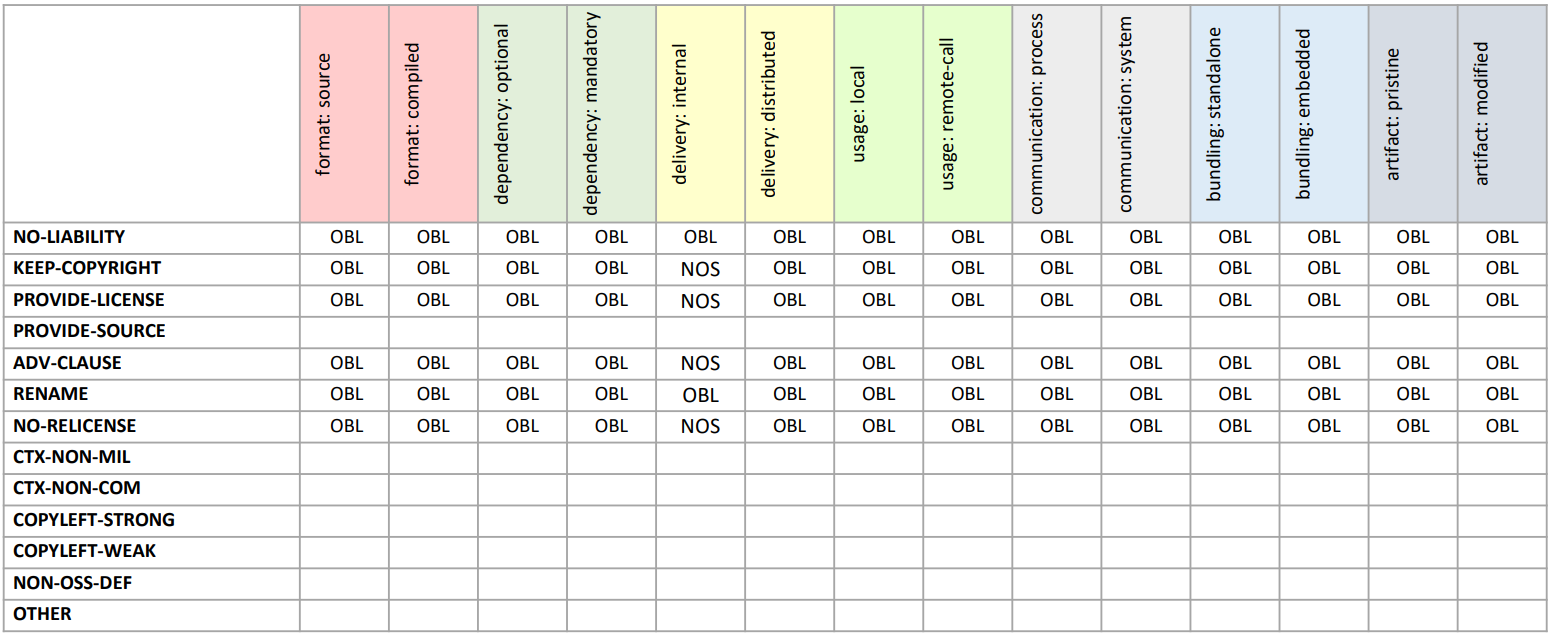
\includegraphics[angle=90, scale=1.0]{Bilder/Manuelle Checkliste.png}
    \caption{Umfassende manuelle Checkliste}
\end{figure}

\newpage
\paragraph{3.3.3.1. Komprimierung der manuellen Checkliste}

Um eine bessere Übersicht über die wesentlichen Elemente zu gewinnen, wurde in diesem Schritt die manuelle Checkliste komprimiert, indem Spalten mit den Ausprägungen die keine Verpflichtungen aufgewiesen haben, entfernt wurden. Damit wird das Ziel verfolgt, eine möglichst leicht verständliche und übersichtliche Checkliste zu generieren, indem nur die wesentlichen Elemente eines Lizenzmodells angezeigt werden. 

\begin{figure}[h]
    \centering
    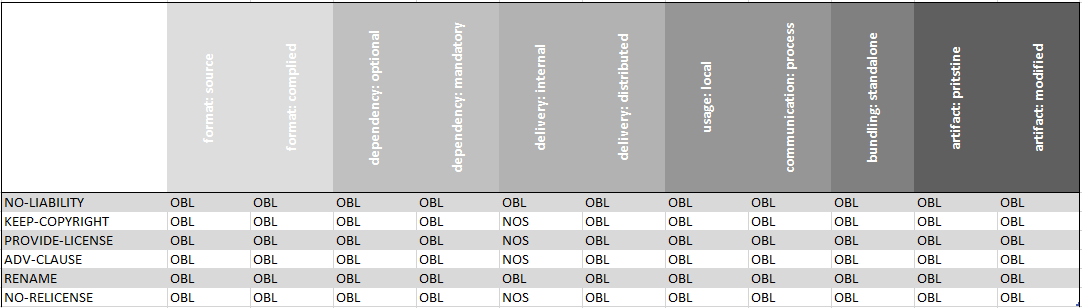
\includegraphics[scale=0.6]{Bilder/Manuelle Checkliste_komprimiert.png}
    \caption{Komprimierte manuelle Checkliste basierend auf der Apache Licence 2.0}
\end{figure}





% Diese Checkliste wurde mit einigen Kollegen der msg systems ag zusammengestellt und entwickelt. dh Ralf und Navina erwähnen 